\section{System Design}
\label{sec:system_design}
The proposed system architecture is a hardware/software co-design framework to investigate tensor acceleration targeting embedded FPGAs. In this paper, we focus on the base embedded system architecture with a single TP. The software and hardware architectures are shown in \Fig{fig:system_architecture} and \Fig{fig:sw_stack}, respectively.

\begin{figure}[t!]
	\centering
	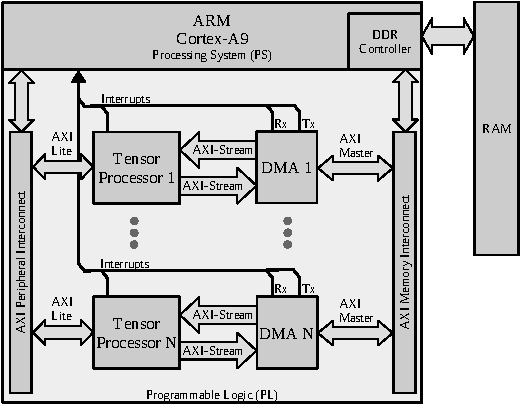
\includegraphics[width=0.5\textwidth]{../figures/system_design.pdf}
	\caption{Base embedded system architecture.}
	\label{fig:system_architecture}
\end{figure}

\begin{figure}[t!]
	\centering
	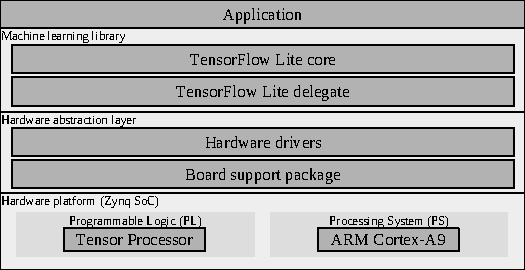
\includegraphics[width=0.5\textwidth]{../figures/sw_stack.pdf}
	\caption{Base embedded software architecture.}
	\label{fig:sw_stack}
\end{figure}

\paragraph{\textbf{Tensor processor}}
The TP is a dedicated hardware module to compute tensor operations. The hardware architecture is described in \fig{fig:accelerator}. This architecture implements high performance off-chip communication with AXI-Stream, direct CPU communication with AXI-Lite, and on-chip storage utilizing BRAM. This hardware architecture is implemented with HLS. The tensor operations are implemented based on the C++ TF Lite micro kernels \cite{tfLiteMicro}.


\begin{eqnarray} \label{eq:tp_memory}
TP_{M}=Input_{M}+Filter_{M}+Bias_{M}+Var_{M}
\end{eqnarray}	

\begin{eqnarray} \label{eq:input_memory}
Input_{M}=K_{H}W_{I}C_{I}BitSize_{I}
\end{eqnarray}

\begin{eqnarray} \label{eq:filter_memory}
Filter_{M}=C_{I}K_{W}K_{H}C_{O}BitSize_{F}
\end{eqnarray}

\begin{eqnarray} \label{eq:bias_memory}
Bias_{M}=C_{O}BitSize_{B}
\end{eqnarray}

\begin{eqnarray} \label{eq:channel_in_memory}
C_{O}=\frac{TP_{M}-Var_{M}-K_{H}W_{I}C_{I}BitSize_{I}}{C_{I}K_{W}K_{H}BitSize_{F}+BitSize_{B}}
\end{eqnarray}

\begin{figure}[h!]
	\centering
	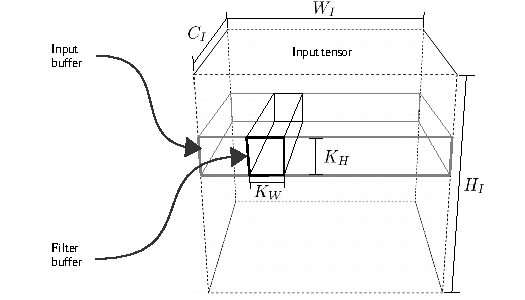
\includegraphics[width=0.5\textwidth]{../figures/accelerator_buffers.pdf}
	\caption{Convolution of input tensor illustrating filter buffer and input buffer.}
	\label{fig:accelerator_buffers}
\end{figure}

\begin{figure}[h!]
	\centering
	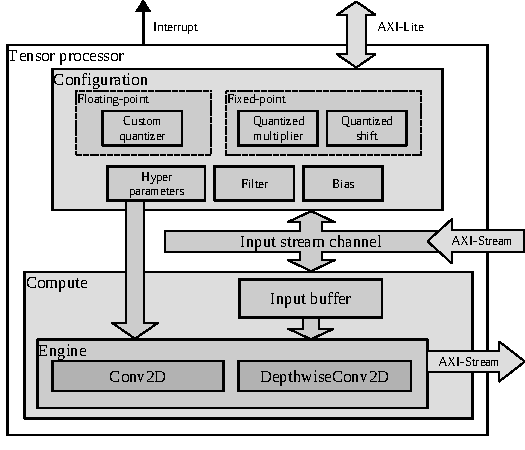
\includegraphics[width=0.5\textwidth]{../figures/accelerator.pdf}
	\caption{Hardware architecture of the proposed tensor processor.}
	\label{fig:accelerator}
\end{figure}

\paragraph{\textbf{Modes of operation}} This accelerator offers two modes of operation: \emph{configuration} and \emph{execution}.

In \emph{configuration} mode, the TP receives the operation ID and hyperparameters: stride, dilation, padding, offset, activation, quantized activation, depth-multiplier, input shape, filter shape, bias shape, and output shape. Afterwards, the TP receives filter and bias tensors to be locally stored.

In \emph{execution} mode, the TP executes the tensor operator according to the hyperparameters given in the configuration mode. During execution, the input and output tensor-buffers are moved from/to the TF Lite memory regions via direct memory access (DMA).

\paragraph{\textbf{Compatibility}}

 This TP is compatible with TF Lite 8-bit quantized models and standard floating-point. For this purpose, we implement the compute engines with regular fixed-point and floating-point LogiCORE IPs.
 Vivado HLS accomplishes floating-point arithmetic operations by mapping
 them onto Xilinx LogiCORE IP in the resultant RTL \cite{hrica2012floating}.
 
\paragraph{\textbf{Dot-product with floating-point optimization}}
\label{sec:dot_product}
We optimize the floating-point computation adopting the dot-product with hybrid custom floating-point and logarithmic approximation\cite{nevarez2021accelerating}. This approach: (1) denormalizes input numbers, (2) executes computation with integer format for exponent and mantissa, and finally, (3) it normalizes the result into IEEE 754 format. This design implements a pipelined vector dot-product with a latency of $2N+II$ (clock cycles), where $N$ and $II$ are the vector length and initiation interval, respectively. This implementation achieves up to $5\times$ latency reduction compared with a pipelined vector dot-product using Xilinx floating-point LogiCORE \cite{nevarez2021accelerating}. The hardware dot-product is illustrated in \Fig{fig:dot_product}. As a design parameter, the mantissa bit-width of the weight vector provides a tunable knob to trade-off between resource-efficiency and QoR \cite{park2009dynamic}. Since the lower-order bits have smaller significance than the higher-order bits, truncating them may
have only a minor impact on QoR \cite{mittal2016survey}.

\begin{figure}[t!]
	\centering
	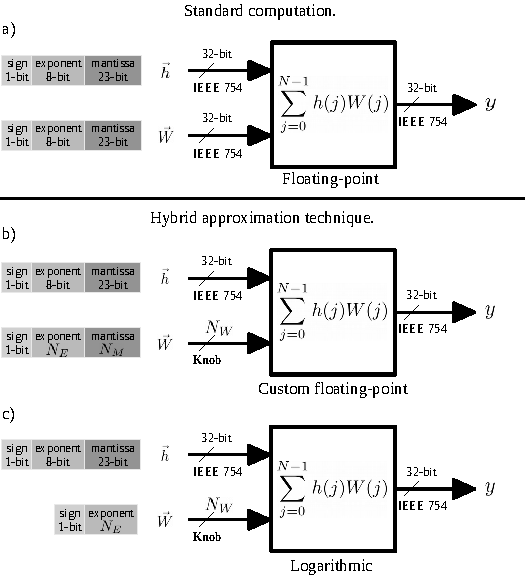
\includegraphics[width=0.5\textwidth]{../figures/dot-product_unit.pdf}
	\caption{Hardware alternatives for vector dot-product.}
	\label{fig:dot_product}
\end{figure}


\paragraph{\textbf{Quantized aware training}}


\begin{algorithm}[h!]
	\label{alg:quantize_training}
	\caption{Custom floating-point quantization.}
	\begin{algorithmic}
		\SetAlgoLined
		\renewcommand{\algorithmicrequire}{\textbf{input:}}
		\renewcommand{\algorithmicensure}{\textbf{output:}}
		\REQUIRE $MODEL$ as the CNN.
		\REQUIRE $E_{size}$ as the target bit size for exponent.
		\REQUIRE $M_{size}$ as the target bits size for mantissa.
		\REQUIRE $STDM_{size}$ as the IEEE 754 bits size for mantissa.
		\FOR {$layer$ in $MODEL$}
		\IF {$layer$ is $Conv2D$ or $SeparableConv2D$}
		\STATE GET FILTER TENSOR $filter \gets Filter(layer)$
		\STATE GET BIAS TENSOR $bias \gets Bias(layer)$
		\FOR {$x$ in $filter$ and $bias$}
			\STATE $sign \gets Sign(x)$
			\STATE $exp \gets Exponent(x)$
			\STATE $fullexp \gets 2^{E_{size}-1}-1$ // Full range value of exp
			\STATE $cman \gets CustomMantissa(x, M_{size})$
			\STATE $resman \gets ResidualMantissa(x, M_{size})$
			\IF {$exp <-fullexp$}
				\STATE$x\gets0$
			\ELSIF{$exp > fullexp$}
				\STATE$x\gets (-1)^{sign}\cdot2^{fullexp}\cdot(1+(1-2^{-M{size}}))$
			\ELSE
				\IF {$2^{STDM_{size}-M_{size}-1}-1<resman$}
					\STATE $cman \gets cman+1$
					\IF{$2^{M_{size}}-1<cman$}
					\STATE $cman \gets 0$
					\STATE $exp \gets exp + 1$
					\ENDIF
				\ENDIF
				\STATE$x\gets (-1)^{sign}\cdot2^{exp}\cdot(1+cman\cdot2^{-M_{size}})$
			\ENDIF
		\ENDFOR		
		\ENDIF
		\ENDFOR
	\end{algorithmic}
\end{algorithm}

